\documentclass{article}

\usepackage[utf8]{inputenc}
\usepackage[letterpaper, total={6in, 9in}]{geometry}
\usepackage{amsmath}
\usepackage{natbib}
\usepackage{wrapfig}
\usepackage{graphicx}
\usepackage{amssymb}
\usepackage{tikz}

\title{Geometry 5 - 3D Geometry Intro}
\author{TSS Math Club}
\date{Dec 2022}

\begin{document}
\large

\maketitle

\section{3D Geometry: Think 2D}

\subsection{Example}

In a regular tetrahedron $ABCD$, $M$ is the midpoint of $CD$. Find $\angle AMB$.



\tikzset{every picture/.style={line width=0.75pt}} %set default line width to 0.75pt        

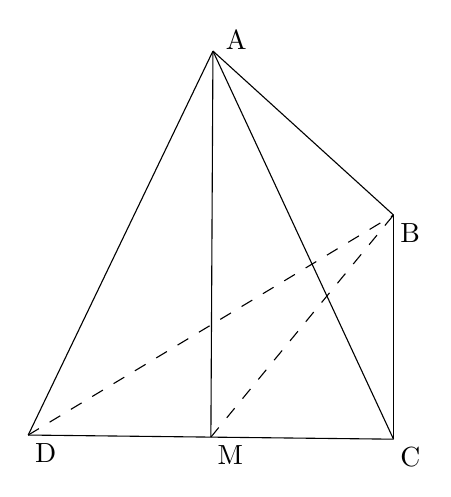
\begin{tikzpicture}[x=0.75pt,y=0.75pt,yscale=-1,xscale=1]
%uncomment if require: \path (0,411); %set diagram left start at 0, and has height of 411

%Straight Lines [id:da34272227772330743] 
\draw    (195.06,89.03) -- (106.06,274.03) ;
%Straight Lines [id:da3339173174782286] 
\draw    (282.06,276.03) -- (106.06,274.03) ;
%Straight Lines [id:da5995848735191855] 
\draw    (195.06,89.03) -- (282.06,276.03) ;
%Straight Lines [id:da28532109602059497] 
\draw    (282.06,168.03) -- (282.06,276.03) ;
%Straight Lines [id:da4649549223878937] 
\draw    (195.06,89.03) -- (282.06,168.03) ;
%Straight Lines [id:da7883950536868969] 
\draw  [dash pattern={on 4.5pt off 4.5pt}]  (106.06,274.03) -- (282.06,168.03) ;
%Straight Lines [id:da8940406459523287] 
\draw  [dash pattern={on 4.5pt off 4.5pt}]  (194.06,275.03) -- (282.06,168.03) ;
%Straight Lines [id:da2799627124005615] 
\draw    (195.06,89.03) -- (194.06,275.03) ;

% Text Node
\draw (200.06,78.03) node [anchor=north west][inner sep=0.75pt]   [align=left] {A};
% Text Node
\draw (284.06,171.03) node [anchor=north west][inner sep=0.75pt]   [align=left] {B};
% Text Node
\draw (284.06,279.03) node [anchor=north west][inner sep=0.75pt]   [align=left] {C};
% Text Node
\draw (108.06,277.03) node [anchor=north west][inner sep=0.75pt]   [align=left] {D};
% Text Node
\draw (196.06,278.03) node [anchor=north west][inner sep=0.75pt]   [align=left] {M};


\end{tikzpicture}

\pagebreak

\subsection{Example}
In the diagram, $PABCD$ is a pyramid with square base $ABCD$ and with $PA = PB = PC = PD$.
Suppose that $M$ is the midpoint of $PC$ and that
$\angle BMD = 90^{\circ}$
. Triangular-based pyramid $MBCD$ is
removed by cutting along the triangle defined by the
points $M$, $B$ and $D$. The volume of the remaining
solid $PABMD$ is 288. What is the length of $AB$?



\tikzset{every picture/.style={line width=0.75pt}} %set default line width to 0.75pt        

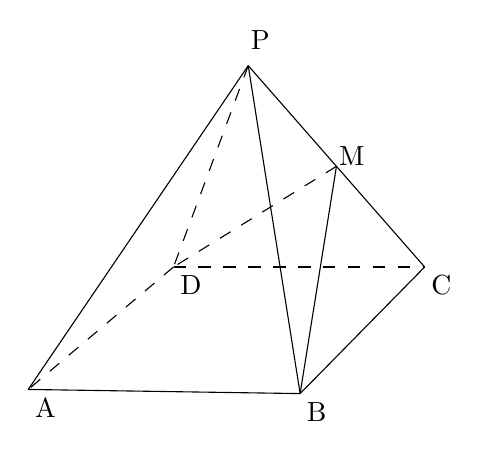
\begin{tikzpicture}[x=0.75pt,y=0.75pt,yscale=-1,xscale=1]
%uncomment if require: \path (0,411); %set diagram left start at 0, and has height of 411

%Straight Lines [id:da06642841678963718] 
\draw    (365.01,240.03) -- (305.01,301.03) ;
%Straight Lines [id:da3133032105153588] 
\draw    (174.01,299.03) -- (305.01,301.03) ;
%Straight Lines [id:da6284514265613841] 
\draw  [dash pattern={on 4.5pt off 4.5pt}]  (244.01,240.03) -- (174.01,299.03) ;
%Straight Lines [id:da23993957607006688] 
\draw    (280.01,143.03) -- (365.01,240.03) ;
%Straight Lines [id:da7607172045026722] 
\draw  [dash pattern={on 4.5pt off 4.5pt}]  (244.01,240.03) -- (365.01,240.03) ;
%Straight Lines [id:da541146629296426] 
\draw    (280.01,143.03) -- (305.01,301.03) ;
%Straight Lines [id:da48648394482635626] 
\draw    (280.01,143.03) -- (174.01,299.03) ;
%Straight Lines [id:da3430468133518938] 
\draw  [dash pattern={on 4.5pt off 4.5pt}]  (280.01,143.03) -- (244.01,240.03) ;
%Straight Lines [id:da3660616410952906] 
\draw  [dash pattern={on 4.5pt off 4.5pt}]  (322.51,191.53) -- (244.01,240.03) ;
%Straight Lines [id:da1892378151273295] 
\draw    (322.51,191.53) -- (305.01,301.03) ;

% Text Node
\draw (176.01,302.03) node [anchor=north west][inner sep=0.75pt]   [align=left] {A};
% Text Node
\draw (307.01,304.03) node [anchor=north west][inner sep=0.75pt]   [align=left] {B};
% Text Node
\draw (367.01,243.03) node [anchor=north west][inner sep=0.75pt]   [align=left] {C};
% Text Node
\draw (246.01,243.03) node [anchor=north west][inner sep=0.75pt]   [align=left] {D};
% Text Node
\draw (280,125) node [anchor=north west][inner sep=0.75pt]   [align=left] {P};
% Text Node
\draw (322.51,180.53) node [anchor=north west][inner sep=0.75pt]   [align=left] {M};


\end{tikzpicture}

\pagebreak

\subsection{Example}
Three spheres with radii $11$, $13$, and $19$ are mutually externally tangent. A plane intersects the spheres in three congruent circles centered at $A$, $B$, and $C$, respectively, and the centers of the spheres all lie on the same side of this plane. Suppose that $AB^2 = 560$. Find $AC^2$

\end{document}